\newpage
\section{Liveness(活跃性) Analysis}
\subsection{Definition}
% \begin{definition}
%     A variable is \textbf{live} if it holds a value that may be needed in the future.
% \end{definition}
编译器需要分析程序的中间表示,以确定那些临时变量在同时被使用.如果一个变量的值在将来还需要使用,则变量是活跃的 (live),这种分析叫做活跃分析.

控制流图(control flow graph): 程序的每条语句都是流图的节点.


\begin{figure}[!htb]
    \centering
    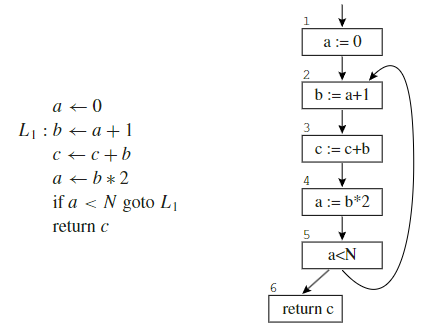
\includegraphics[width=0.309\textwidth]{pic/CP10/Control-flow graph of a program}
    \caption{Control-flow graph of a program}
\end{figure}


活跃范围(Liveness): 变量位索引的集合,变量在那几条边上活跃的边集合.

\begin{figure}[!htb]
    \centering
    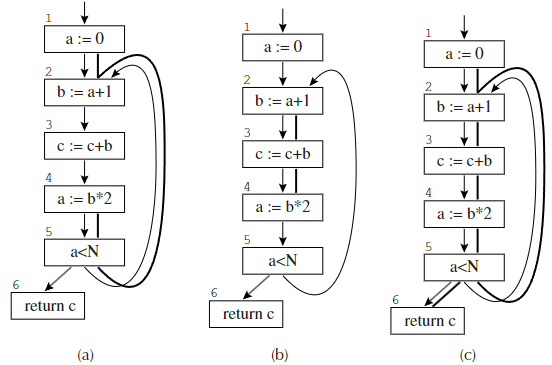
\includegraphics[width=0.42\textwidth]{pic/CP10/Liveness of variables}
    \caption{Liveness of variables $a, b, c$.}
\end{figure}

\subsection{Solution of Dataflow Equations}

\begin{itemize}
    \item 出边(out-edge):节点引向后继节点的边; 
    \item 入 边 (in-edge): 由 前 继 节 点 指 向 的边.
\end{itemize}
$succ[n]$ 是节点 $n$ 的后继节点; $pred[n]$ 是节点 $n$ 的前驱节点


\begin{itemize}
    \item 定义(define): 对变量和临时变量的赋值称为变量的定义;
    \item 使用(use): 使用出现在赋值号右边的变量.
\end{itemize}

活跃性(Liveness): 变量在边上活跃是指存在一条边通向一个使用该变量的有向路径,且不经过该变量的任何定义.
\begin{itemize}
    \item 如果变量在一个节点的所有入边上全是活跃的,那么该变量是入口 活 跃 的 (live-in); 
    \item 若 一个变量在一个节点的所有出边上都是活跃的,那么该变量在 该 节 点 是 出 口 活 跃 的(live-out).
\end{itemize}

\subsubsection{Calculation of Liveness}
就是计算流图每一个节点的 $in$ 和 $out$ 集合
\begin{equation}
    \begin{split}
        in[n]&=use[n]\cup (out[n]-def[n])\\
        out[n]&=\bigcup_{s\in succ[n]}in[s]
    \end{split}\label{eq:liveness}
\end{equation}

活跃性计算的迭代方法
\begin{algorithm}[H]
    \caption{Computation of liveness by iteration}
    \label{algo:liveness}
    \begin{algorithmic}
        \For{each $n$}
            \State $in[n]\leftarrow \{\};\ out[n]\leftarrow \{\}$
        \EndFor
        \Repeat
            \For{each $n$}
                \State $in'[n]\leftarrow in[n];\ out'[n]\leftarrow out[n]$
                \State $in[n]\leftarrow use[n] \cup (out[n] - def[n])$
                \State $\displaystyle out[n]\leftarrow \bigcup_{s\in succ[n]}in[s]$
            \EndFor
        \Until{$in'[n]=in[n]$ and $out'[n]=out[n]$ for all $n$}
    \end{algorithmic}
\end{algorithm}

\begin{figure}[!htb]
    \centering
    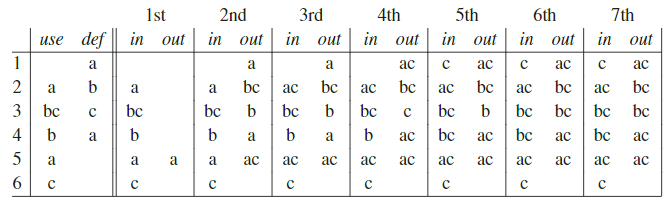
\includegraphics[height=0.14\textwidth]{pic/CP10/Liveness calculation following forward control-flow edges.}
    \caption{Liveness calculation following forward control-flow edges.}
\end{figure}

\begin{figure}[!htb]
    \centering
    \includegraphics[height=0.14\textwidth]{pic/CP10/Liveness calculation following reverse control-flow edges}
    \caption{Liveness calculation following reverse control-flow edges.}
\end{figure}

适当排序可以显著加快算法的收敛过程,一般要从程序末尾往前算,先算 $out$ 再算 $in$,可以显著提高速度和正确率. 信息活跃性是沿控制流箭头的反方向流动的,计算顺序同理.


时间复杂度: 
\begin{itemize}
    \item for 循环初始化 节 点 $in,out$ 需 要 $O(N^2)$; 
    \item repeat 循环 的时 间复杂度是 $O(N^4)$.
\end{itemize}
由于活跃信息大部分稀疏,实际运行时间在 $O(N)$ 和 $O(N^2)$ 之间.

\subsubsection{Representation of Sets}
\begin{itemize}
    \item 位数组(bit array): 程序中有 $N$ 个变量,用 $N$ 位二进制数表示集合
    \subitem 求并集对位数组求按位或
    \subitem 时间效率:对每个字有 $K$ 位的计算机, 并运算需要 $N/K$ 次操作
    \item 有序变量表:链表的成员是组成集合的元素
    \subitem 并集通过合并链表实现
    \subitem 时间开销和求并集的集合大小成线性.
\end{itemize}

集合稀疏(平均少于 $N/K$)用有序链表表示速度会更快(越稀疏越快); 集合密集位数组表示更好.

\subsubsection{Least Fixed Points}
\textbf{Equation} \ref{eq:liveness} 的解只是保守的近似解,只能保证生成的代码是正确的, 但是所使用的寄存器可能比实际需要的多. 

\begin{theorem}
    \textbf{Equation} \ref{eq:liveness} 有一个以上的解.
\end{theorem}
\begin{proof}
    增加更多的变量后, 结果仍是 \textbf{Equation} \ref{eq:liveness} 的解.
\end{proof}

\begin{theorem}
    \textbf{Equation} \ref{eq:liveness} 的所有解都包含最小解(least solution). 
\end{theorem}

\textbf{Algorithm} \ref{algo:liveness} 所计算的就是最小解. 

\subsubsection{Static v.s. Dynamic Liveness}
\begin{theorem}[Halting Problem]
    不存在程序 $H$, 其以任意程序 $P$ 和 输入 $X$ 作为自己的输入. 当 $P(X)$ 停止时返回真, 否则返回假. 
\end{theorem}

\begin{corollary}
    不存在程序 $H'(X, L)$, 对任何程序 $X$ 和其中标记 $L$, 可以判断 $X$ 在执行中是否到达过 $L$.
\end{corollary}
意思是不存在一个通用程序能算出每一个标记是否达到. 


动态判断及其静态的近似:
\begin{itemize}
    \item 动态活跃(Dynamic liveness): 如果程序从节点 $n$ 执行到 使用 $a$ 之间没有经过 $a$ 的任何 定义,那么变量 $a$ 在节点 $n$ 是动态活跃的.
    \item 静态活跃(Static liveness): 如果存在着一条从 $n$ 到 使用 $a$ 的控制流路径,且此路径上没有 $a$ 的任何 定义,那么变量 $a$ 在节点 $n$ 静态活跃的.
\end{itemize}

\subsubsection{Interference Graphs}
\begin{definition}
    两个临时变量不能分配到同一个寄存器的情况称为冲突(interference).
\end{definition}

冲突原因:
\begin{enumerate}
    \item 临时变量在程序的同一点同时活跃
    \item 某些寄存器必须被使用时,临时变量不能占用这些寄存器.
\end{enumerate}

\begin{figure}[!htb]
    \centering
    \begin{subfigure}{0.12\textwidth}
        \centering
        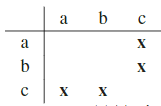
\includegraphics[width=\textwidth]{pic/CP10/Matrix.png}
        \caption{Matrix}
    \end{subfigure}
    \begin{subfigure}{0.08\textwidth}
        \centering
        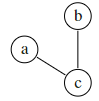
\includegraphics[width=\textwidth]{pic/CP10/Graph.png}
        \caption{Graph}
    \end{subfigure}
    \caption{Representations of interference}
\end{figure}

绘制冲突图的办法:为新定义 (def) 添 加 冲 突 边 的 办 法是
\begin{enumerate}
    \item 对 变 量 $a$ 非 MOVE 指令的定义 , 以及在该指令节 点 $n$ 处,任意 $b_i\in out[n]$,添 加 冲 突 边 $(a,b_i)$
    \item 对 于 节 点标号为 $n$ 的 MOVE 指令 $a\leftarrow c$,对 $b_i\in out[n]$ 且 $b_i\ne c$, 添加边 $(a,b_i)$. 
\end{enumerate}
注:可以给 $(a,c)$ 画上虚线,便于寄存器 分配的 coalesce.


